\chapter{Introduction}
\setlength{\epigraphwidth}{0.7\textwidth}
\renewcommand{\epigraphflush}{center}
\epigraph{\textit{Any function of independent random variables that depends on many of them, but not too much on each of them, is essentially constant.}}{Talagrand}
\section{About Concentration Inequalities}
Starting with one of the most fundamental result:
\begin{theorem}[Weak Law of Large Numbers]
Say $X_i$'s are i.i.d. random variables with $\EE[X_i] < \infty$, and denote $Z = \frac{\sum_{i=1}^n X_i}{n}$. Then,
\begin{equation}\label{eq:wlln}
    \forall \epsilon > 0, \quad \lim_{n\to\infty} \PP(|Z - \EE[Z]| > \epsilon) = 0
\end{equation}
\end{theorem}
Two things to note about this are: $(1)$ $Z$ is a sum of $n$ i.i.d. random variables, and $(2)$ The statement is asymptotic. We will proceed forward with the following goals in mind: $(1)$ We want to extend ideas to more general functions, $(2)$ We want to relax the i.i.d. assumption, and $(3)$ We want to quantify what \textit{essentially constant} means. \\
Concentration inequalities often take the form (or an extended variant to include multiple random variables): $\PP(|X - \EE[X]| > \epsilon) \leq g(\epsilon)$. \\
It becomes necessary to study concentration inequalities, as often the characterization of the left-hand is difficult, such inequalities pop-up in analysis, design and inference of randomized algorithms, and moreover in predictions or hypothesis testing.
\begin{eg}[Design]
Consider a party where $n$ people are invited. Ideally, you would require $n$ chairs in a room to accomodate everyone. However, it is known that not everyone shows up at the party. Consider the following model: Let each person show up with probability $p$. We would also like to consider some risk $\delta \in (0,1)$, and we would want that w.p. $\geq 1-\delta$: everyone who shows up gets a seat. Consider for person $i$:
\[
X_i = \begin{cases}
    1 & \text{if the person shows up} \\
    0 & \text{otherwise}
\end{cases}
\]
and $X = \sum_i X_i$. Let us model the deviation from the mean $\EE[X] = np$, as $\PP(X > \EE[X] + t) \leq e^{-\frac{2t^2}{n}}$
Setting $\delta = e^{-\frac{2t^2}{n}}$ gives us $t = \sqrt{\frac{n}{2} \log\frac{1}{\delta}}$. This gives us the following for $p=0.5$ and $n=100$:
\begin{table}[H]
    \centering
    \begin{tabular}{c|c|c|c}
         & $\delta=0.1$ & $\delta=0.01$ & $\delta=0.001$\\ \hline
        $\lceil\EE[X]+t\rceil$ & 61 & 66 & 69\\
    \end{tabular}
    \caption{Variation of number of chairs with risk $\delta$}
    \label{tab:eg1}
\end{table}
\end{eg}
\begin{eg}[Inference]
Consider a biased coin, with an unknown $\PP(\text{heads}) = p$. We toss the coin $n$ times and $n_H$ heads are obtained. How to compute $p_\text{max}$ such that $\PP(p > p_\text{max}) \leq \delta$?
\end{eg}
\section{Basic Inequalities}
\begin{theorem}[Markov's Inequality]
Say $X$ is a non-negative random variable, and $\EE[X] < \infty$. Then, for $\alpha > 0$,
\begin{equation}
    \PP(X > \alpha) \leq \frac{\EE[X]}{\alpha}
\end{equation}
\end{theorem}
\begin{proof}
\[
\EE[X] = \int_0^\infty x f_X(x) dx = \underbrace{\int_0^\alpha xf_X(x)dx}_{\geq 0} + \underbrace{\int_\alpha^\infty x f_X(x) dx}_{\geq \alpha \PP(X>\alpha)}
\]
\end{proof}
\begin{eg}
For $X \sim \text{Exp}(\lambda)$, $\EE[X] = \frac{1}{\lambda}$. By Markov's Inequality, we have $\PP(X > \alpha) \leq \frac{1}{\lambda \alpha}$, which gives a linear decay. However, we can explicitly calculate $\PP(X > \alpha) = e^{-\lambda \alpha}$ -- which is an exponential decay and hence in this case, Markov's Inequality gives a much weaker result than the true value.
\end{eg}
\begin{theorem}[Chebyshev's Inequality]
   Say $X$ is a random variable with mean $\mu$ and variance $\sigma^2$. Then, for $\alpha > 0$,
   \begin{equation}
       \PP(|X - \EE[X]| > \alpha) \leq \frac{\sigma^2}{\alpha^2}
   \end{equation}
\end{theorem}
\begin{proof}
Let $Y = |X - \EE[X]|$. Then,
\[
\PP(Y > \alpha) \stackrel{*}{\leq} \PP(Y^2 > \alpha^2) \stackrel{**}{\leq}\frac{\EE[Y^2]}{\alpha^2} = \frac{\sigma^2}{\alpha^2}
\]
Note that in this case $(*)$ is infact an equality, and $(**)$ follows from Markov's Inequality.
\end{proof}
Before moving on to the next bound, we note the following: Consider $\PP(X > \alpha)$, and let $f(\cdot)$ be a monotonically increase non-negative function. Then, $\PP(f(X) > f(\alpha)) \leq \frac{\EE[f(X)]}{f(\alpha)}$ follows from Markov's Inequality. In cases where the RHS is tighter than the RHS given by Markov's Inequality, we would like to tighten the bound through such an appropriate function $f$.
\begin{theorem}[Chernoff Bound]
For a random variable $X$, define $\psi_X(s) = \log(\EE[e^{sX}])$ as the log M.G.F., and $\psi_X^*(a) = \sup_{s > 0} (sa - \psi_X(s))$. Then,
\begin{equation}
    \PP(X > \alpha) \leq e^{-\psi_X^*(\alpha)}
\end{equation}
\end{theorem}
\begin{proof}
Let $f(t) = e^{st}$ for $s > 0$. Then through the discussion above, we know that 
\[
\PP(X > \alpha) = \PP(f(X) > f(\alpha)) = \PP(e^{sX} > e^{s\alpha}) \leq \frac{\EE[e^{sX}]}{e^{s\alpha}} = e^{-s\alpha + \log \EE[e^{sX}]}
\]
\end{proof}
where the last inequality follows from Markov's Inequality. Since the RHS doesn't depend on $s$, we can minimize the RHS by taking the supremum over $s$.
\begin{eg}
Let $X \sim \text{Exp}(\lambda)$ for $\lambda > 0$. For $\lambda > s$,
\begin{align*}
    \EE[e^{sX}] &= \int_0^\infty e^{sx}\lambda e^{-\lambda x} dx = \frac{\lambda}{\lambda - s} \implies \psi_X(s) = \log\left(\frac{\lambda}{\lambda - s}\right) \\
    \psi_X^*(\alpha) &= \sup_{0 < s <\lambda} \left(s\alpha - \log\left(\frac{\lambda}{\lambda - s}\right) \right)
\end{align*}
Maximizing this over $s$ gives $s = \lambda - \frac{1}{\alpha}$. Thus, $\psi_X^*(\alpha) = \alpha \lambda - \log (\alpha \lambda) - 1$. Thus, we get
$\PP(X > \alpha) \leq e^{-\psi_X^*(\alpha)} = e\alpha\lambda e^{-\alpha \lambda}$
\begin{figure}[H]
    \centering
    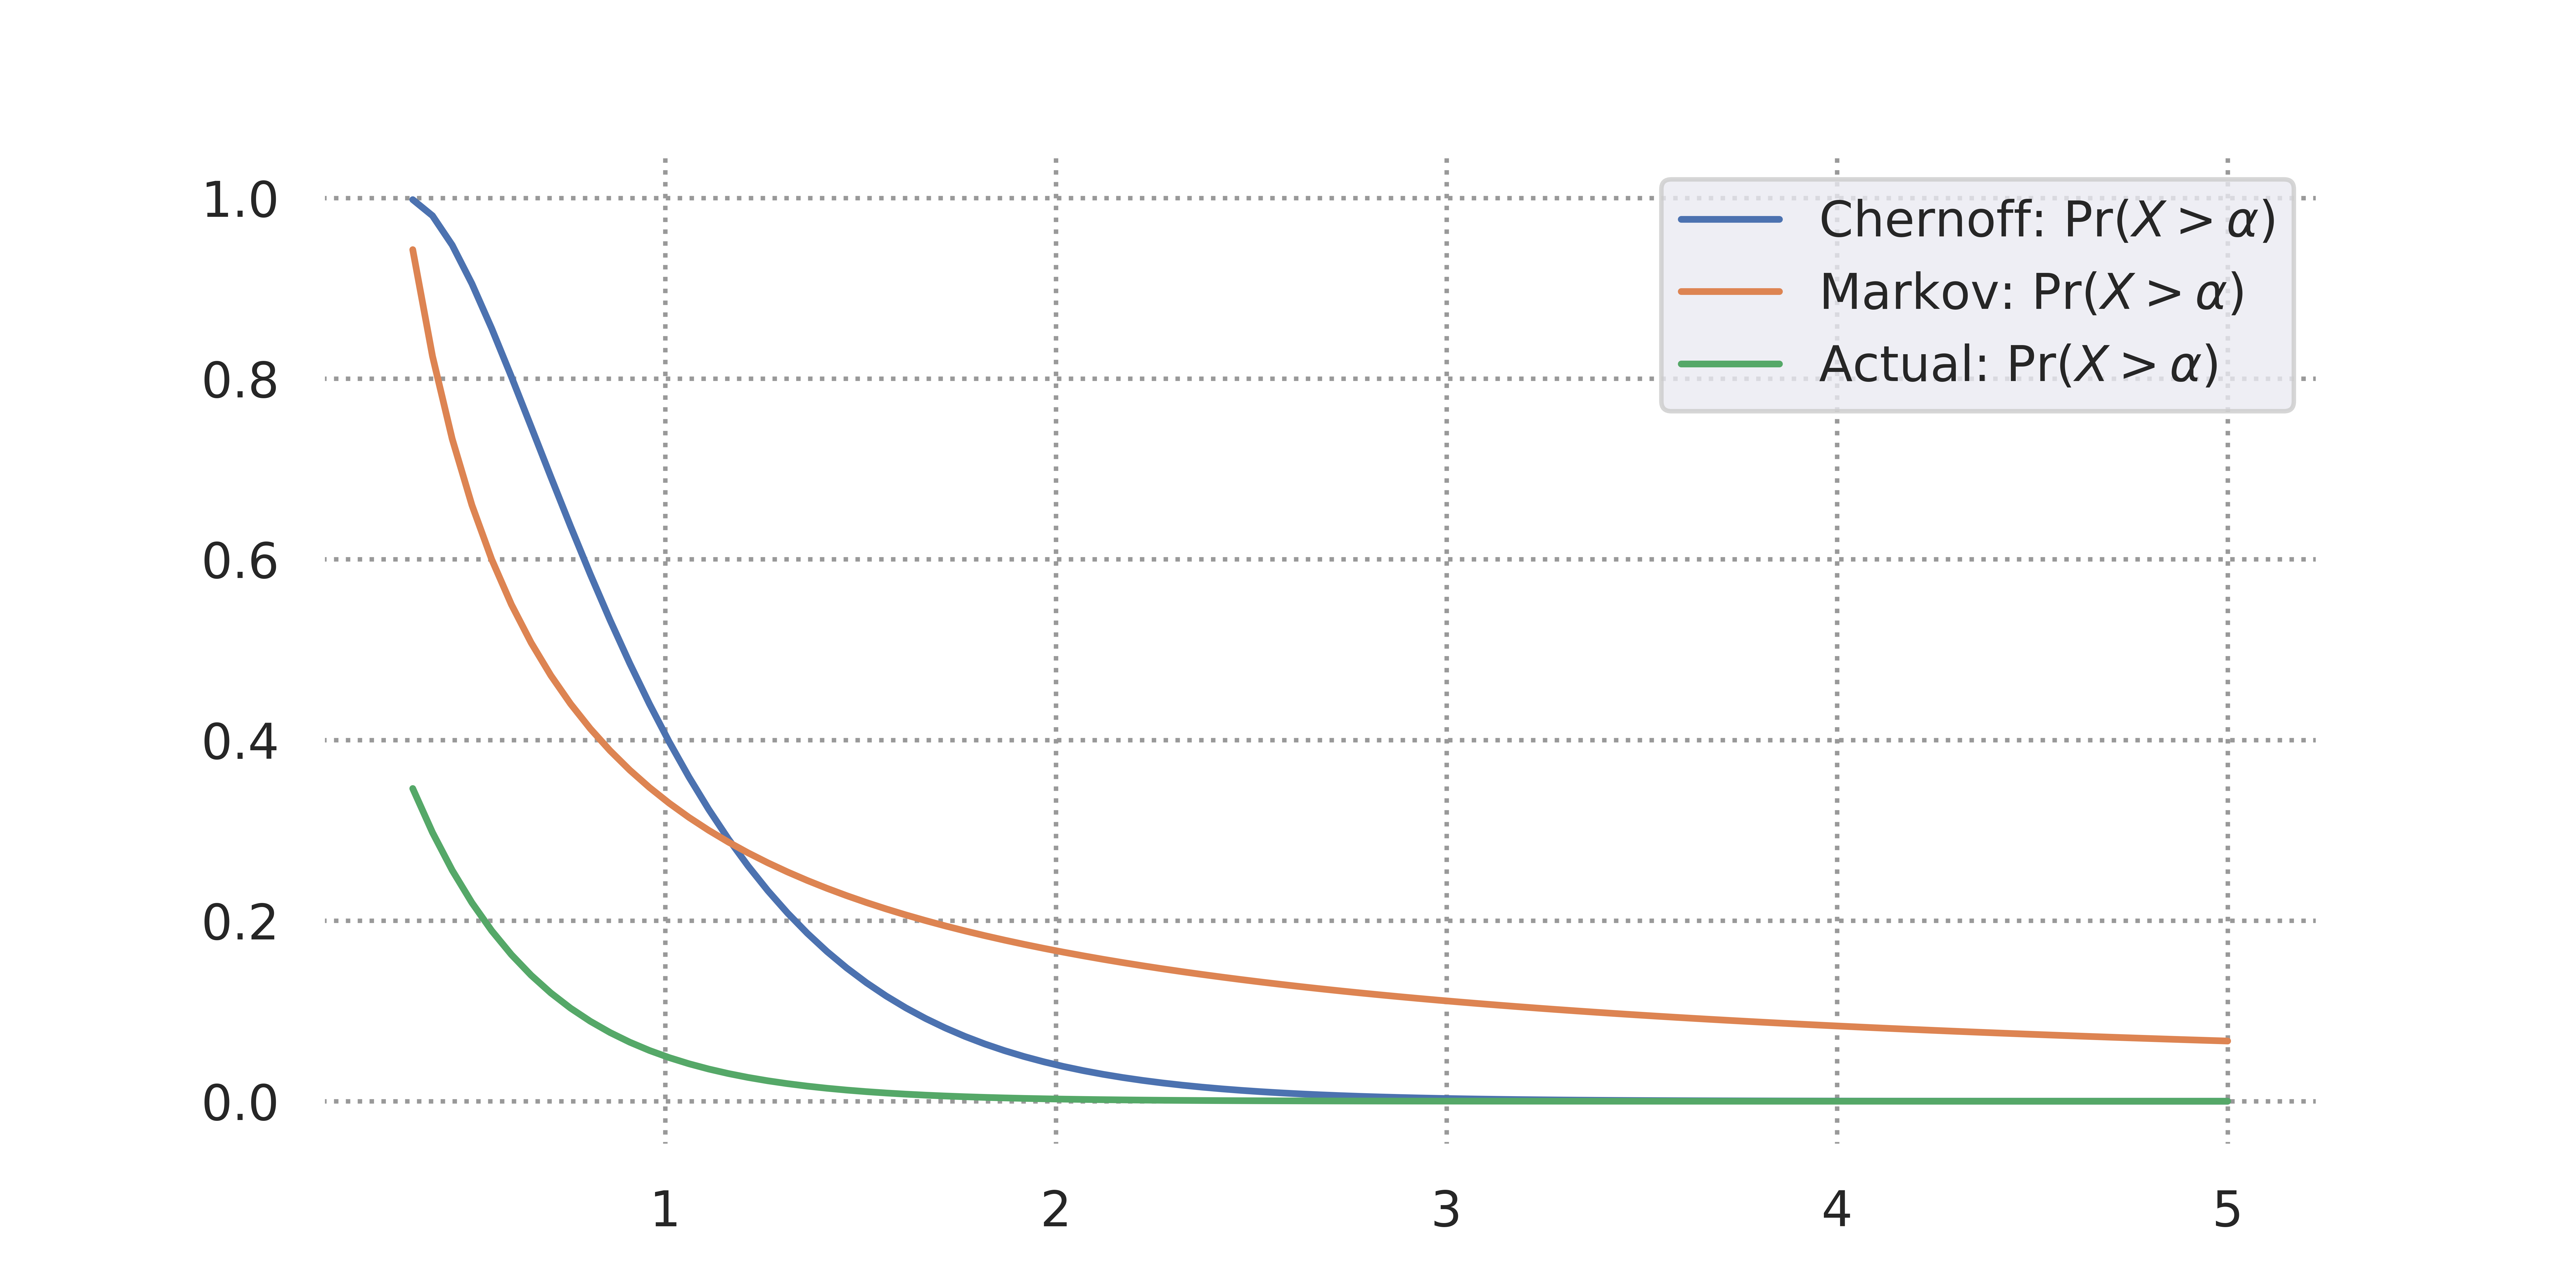
\includegraphics[width=0.8\textwidth]{fig/demo.png}
    \caption{Comparison of bounds for $X\sim\text{Exp}(3)$ for $\alpha > \frac{1}{3}$}
\end{figure}
\end{eg}
\begin{corollary}[Chernoff Bound for sum of i.i.d. random variables]
Let $\{X_i\}_{i=1}^n$ be i.i.d. random variables, and let $Z = \sum_i X_i$. Then, $\EE[e^{sZ}] = (\EE[e^{sX_1}])^n$, and $\psi_Z^*(n\alpha) = n\psi_{X_1}^*(\alpha)$. Thus,
\begin{equation}
    \PP(Z > n\alpha) \leq e^{-n\psi_{X_1}^* (\alpha)}
\end{equation}
\end{corollary}
\begin{hw}
Let $X \sim \text{Bern}(p)$. Then we have:
\[
\psi_X(s) = \log \EE[e^{sX}] = \log\left[\PP(X=0)e^{s \cdot 0} + \PP(X=1)e^{s \cdot 1}\right] = \log\left[ (1-p) + pe^s\right]
\]
Since $\psi_X^*(\alpha) = \sup_{s > 0} \left( s\alpha - \psi_X(s)\right)$, we can find the optimal $s$ as
\begin{align*}
    \alpha - \frac{pe^s}{1-p+pe^s} &= 0 \implies s = \log\left[\left(\frac{\alpha}{1-\alpha}\right) \left(\frac{1-p}{p}\right)\right] \\
\therefore \psi_X^*(\alpha) &=\alpha\log\left[\left(\frac{\alpha}{1-\alpha}\right) \left(\frac{1-p}{p}\right)\right] + \log\left(\frac{1-p}{1-\alpha}\right)
\end{align*}
Recall that for $X_1 \sim \text{Bern}(p_1)$ and $X_2 \sim \text{Bern}(p_2)$, the  Kullback-Leibler divergence of $X_1$ and $X_2$ is given as
\[
\kl{X_1}{X_2} = \sum_{x \in \{0,1\}} \PP(X_1 = x) \log\frac{\PP(X_1=x)}{\PP(X_2=x)} = p_1 \log\frac{p_1(1-p_2)}{p_2(1-p_1)} + \log\frac{1-p_1}{1-p_2}
\]
Thus, $\psi_X^*(\alpha) = \kl{\text{Bern}(\alpha)}{X}$, which gives 
\[
\PP(X > \alpha) \leq \left(\frac{p}{\alpha}\right)^{\alpha} \left(\frac{1-p}{1-\alpha}\right)^{1-\alpha}
\]
\end{hw}
\begin{hw}
Let $X \sim \text{Poi}(\lambda)$. Then, we have
\[
\psi_X(s) = \log \EE[e^{sX}] = \log\left[\sum_{k = 0}^\infty \PP(X=k)e^{sk}\right] = \log\left[e^{-\lambda}\sum_{k=0}^\infty \frac{(\lambda e^s)^k}{k!}\right] = \lambda (e^s - 1) 
\]
Since $\psi_X^*(\alpha) = \sup_{s > 0} \left( s\alpha - \psi_X(s)\right)$, we can find the optimal $s$ as
\begin{align*}
    \alpha - \lambda e^{s} &= 0 \implies s = \log\frac{\alpha}{\lambda} \\
\therefore \psi_X^*(\alpha) &=\alpha\log\frac{\alpha}{\lambda} - \alpha + \lambda \implies \PP(X > \alpha) \leq \left(\frac\lambda\alpha\right)^\alpha e^{\alpha - \lambda}
\end{align*}
\end{hw}